% Generated by Sphinx.
\def\sphinxdocclass{report}
\documentclass[letterpaper,10pt,english]{sphinxmanual}
\usepackage[utf8]{inputenc}
\DeclareUnicodeCharacter{00A0}{\nobreakspace}
\usepackage{cmap}
\usepackage[T1]{fontenc}
\usepackage{babel}
\usepackage{times}
\usepackage[Bjarne]{fncychap}
\usepackage{longtable}
\usepackage{sphinx}
\usepackage{multirow}


\title{pynoddy Documentation}
\date{March 25, 2014}
\release{}
\author{Florian Wellmann}
\newcommand{\sphinxlogo}{}
\renewcommand{\releasename}{Release}
\makeindex

\makeatletter
\def\PYG@reset{\let\PYG@it=\relax \let\PYG@bf=\relax%
    \let\PYG@ul=\relax \let\PYG@tc=\relax%
    \let\PYG@bc=\relax \let\PYG@ff=\relax}
\def\PYG@tok#1{\csname PYG@tok@#1\endcsname}
\def\PYG@toks#1+{\ifx\relax#1\empty\else%
    \PYG@tok{#1}\expandafter\PYG@toks\fi}
\def\PYG@do#1{\PYG@bc{\PYG@tc{\PYG@ul{%
    \PYG@it{\PYG@bf{\PYG@ff{#1}}}}}}}
\def\PYG#1#2{\PYG@reset\PYG@toks#1+\relax+\PYG@do{#2}}

\expandafter\def\csname PYG@tok@gd\endcsname{\def\PYG@tc##1{\textcolor[rgb]{0.63,0.00,0.00}{##1}}}
\expandafter\def\csname PYG@tok@gu\endcsname{\let\PYG@bf=\textbf\def\PYG@tc##1{\textcolor[rgb]{0.50,0.00,0.50}{##1}}}
\expandafter\def\csname PYG@tok@gt\endcsname{\def\PYG@tc##1{\textcolor[rgb]{0.00,0.27,0.87}{##1}}}
\expandafter\def\csname PYG@tok@gs\endcsname{\let\PYG@bf=\textbf}
\expandafter\def\csname PYG@tok@gr\endcsname{\def\PYG@tc##1{\textcolor[rgb]{1.00,0.00,0.00}{##1}}}
\expandafter\def\csname PYG@tok@cm\endcsname{\let\PYG@it=\textit\def\PYG@tc##1{\textcolor[rgb]{0.25,0.50,0.56}{##1}}}
\expandafter\def\csname PYG@tok@vg\endcsname{\def\PYG@tc##1{\textcolor[rgb]{0.73,0.38,0.84}{##1}}}
\expandafter\def\csname PYG@tok@m\endcsname{\def\PYG@tc##1{\textcolor[rgb]{0.13,0.50,0.31}{##1}}}
\expandafter\def\csname PYG@tok@mh\endcsname{\def\PYG@tc##1{\textcolor[rgb]{0.13,0.50,0.31}{##1}}}
\expandafter\def\csname PYG@tok@cs\endcsname{\def\PYG@tc##1{\textcolor[rgb]{0.25,0.50,0.56}{##1}}\def\PYG@bc##1{\setlength{\fboxsep}{0pt}\colorbox[rgb]{1.00,0.94,0.94}{\strut ##1}}}
\expandafter\def\csname PYG@tok@ge\endcsname{\let\PYG@it=\textit}
\expandafter\def\csname PYG@tok@vc\endcsname{\def\PYG@tc##1{\textcolor[rgb]{0.73,0.38,0.84}{##1}}}
\expandafter\def\csname PYG@tok@il\endcsname{\def\PYG@tc##1{\textcolor[rgb]{0.13,0.50,0.31}{##1}}}
\expandafter\def\csname PYG@tok@go\endcsname{\def\PYG@tc##1{\textcolor[rgb]{0.20,0.20,0.20}{##1}}}
\expandafter\def\csname PYG@tok@cp\endcsname{\def\PYG@tc##1{\textcolor[rgb]{0.00,0.44,0.13}{##1}}}
\expandafter\def\csname PYG@tok@gi\endcsname{\def\PYG@tc##1{\textcolor[rgb]{0.00,0.63,0.00}{##1}}}
\expandafter\def\csname PYG@tok@gh\endcsname{\let\PYG@bf=\textbf\def\PYG@tc##1{\textcolor[rgb]{0.00,0.00,0.50}{##1}}}
\expandafter\def\csname PYG@tok@ni\endcsname{\let\PYG@bf=\textbf\def\PYG@tc##1{\textcolor[rgb]{0.84,0.33,0.22}{##1}}}
\expandafter\def\csname PYG@tok@nl\endcsname{\let\PYG@bf=\textbf\def\PYG@tc##1{\textcolor[rgb]{0.00,0.13,0.44}{##1}}}
\expandafter\def\csname PYG@tok@nn\endcsname{\let\PYG@bf=\textbf\def\PYG@tc##1{\textcolor[rgb]{0.05,0.52,0.71}{##1}}}
\expandafter\def\csname PYG@tok@no\endcsname{\def\PYG@tc##1{\textcolor[rgb]{0.38,0.68,0.84}{##1}}}
\expandafter\def\csname PYG@tok@na\endcsname{\def\PYG@tc##1{\textcolor[rgb]{0.25,0.44,0.63}{##1}}}
\expandafter\def\csname PYG@tok@nb\endcsname{\def\PYG@tc##1{\textcolor[rgb]{0.00,0.44,0.13}{##1}}}
\expandafter\def\csname PYG@tok@nc\endcsname{\let\PYG@bf=\textbf\def\PYG@tc##1{\textcolor[rgb]{0.05,0.52,0.71}{##1}}}
\expandafter\def\csname PYG@tok@nd\endcsname{\let\PYG@bf=\textbf\def\PYG@tc##1{\textcolor[rgb]{0.33,0.33,0.33}{##1}}}
\expandafter\def\csname PYG@tok@ne\endcsname{\def\PYG@tc##1{\textcolor[rgb]{0.00,0.44,0.13}{##1}}}
\expandafter\def\csname PYG@tok@nf\endcsname{\def\PYG@tc##1{\textcolor[rgb]{0.02,0.16,0.49}{##1}}}
\expandafter\def\csname PYG@tok@si\endcsname{\let\PYG@it=\textit\def\PYG@tc##1{\textcolor[rgb]{0.44,0.63,0.82}{##1}}}
\expandafter\def\csname PYG@tok@s2\endcsname{\def\PYG@tc##1{\textcolor[rgb]{0.25,0.44,0.63}{##1}}}
\expandafter\def\csname PYG@tok@vi\endcsname{\def\PYG@tc##1{\textcolor[rgb]{0.73,0.38,0.84}{##1}}}
\expandafter\def\csname PYG@tok@nt\endcsname{\let\PYG@bf=\textbf\def\PYG@tc##1{\textcolor[rgb]{0.02,0.16,0.45}{##1}}}
\expandafter\def\csname PYG@tok@nv\endcsname{\def\PYG@tc##1{\textcolor[rgb]{0.73,0.38,0.84}{##1}}}
\expandafter\def\csname PYG@tok@s1\endcsname{\def\PYG@tc##1{\textcolor[rgb]{0.25,0.44,0.63}{##1}}}
\expandafter\def\csname PYG@tok@gp\endcsname{\let\PYG@bf=\textbf\def\PYG@tc##1{\textcolor[rgb]{0.78,0.36,0.04}{##1}}}
\expandafter\def\csname PYG@tok@sh\endcsname{\def\PYG@tc##1{\textcolor[rgb]{0.25,0.44,0.63}{##1}}}
\expandafter\def\csname PYG@tok@ow\endcsname{\let\PYG@bf=\textbf\def\PYG@tc##1{\textcolor[rgb]{0.00,0.44,0.13}{##1}}}
\expandafter\def\csname PYG@tok@sx\endcsname{\def\PYG@tc##1{\textcolor[rgb]{0.78,0.36,0.04}{##1}}}
\expandafter\def\csname PYG@tok@bp\endcsname{\def\PYG@tc##1{\textcolor[rgb]{0.00,0.44,0.13}{##1}}}
\expandafter\def\csname PYG@tok@c1\endcsname{\let\PYG@it=\textit\def\PYG@tc##1{\textcolor[rgb]{0.25,0.50,0.56}{##1}}}
\expandafter\def\csname PYG@tok@kc\endcsname{\let\PYG@bf=\textbf\def\PYG@tc##1{\textcolor[rgb]{0.00,0.44,0.13}{##1}}}
\expandafter\def\csname PYG@tok@c\endcsname{\let\PYG@it=\textit\def\PYG@tc##1{\textcolor[rgb]{0.25,0.50,0.56}{##1}}}
\expandafter\def\csname PYG@tok@mf\endcsname{\def\PYG@tc##1{\textcolor[rgb]{0.13,0.50,0.31}{##1}}}
\expandafter\def\csname PYG@tok@err\endcsname{\def\PYG@bc##1{\setlength{\fboxsep}{0pt}\fcolorbox[rgb]{1.00,0.00,0.00}{1,1,1}{\strut ##1}}}
\expandafter\def\csname PYG@tok@kd\endcsname{\let\PYG@bf=\textbf\def\PYG@tc##1{\textcolor[rgb]{0.00,0.44,0.13}{##1}}}
\expandafter\def\csname PYG@tok@ss\endcsname{\def\PYG@tc##1{\textcolor[rgb]{0.32,0.47,0.09}{##1}}}
\expandafter\def\csname PYG@tok@sr\endcsname{\def\PYG@tc##1{\textcolor[rgb]{0.14,0.33,0.53}{##1}}}
\expandafter\def\csname PYG@tok@mo\endcsname{\def\PYG@tc##1{\textcolor[rgb]{0.13,0.50,0.31}{##1}}}
\expandafter\def\csname PYG@tok@mi\endcsname{\def\PYG@tc##1{\textcolor[rgb]{0.13,0.50,0.31}{##1}}}
\expandafter\def\csname PYG@tok@kn\endcsname{\let\PYG@bf=\textbf\def\PYG@tc##1{\textcolor[rgb]{0.00,0.44,0.13}{##1}}}
\expandafter\def\csname PYG@tok@o\endcsname{\def\PYG@tc##1{\textcolor[rgb]{0.40,0.40,0.40}{##1}}}
\expandafter\def\csname PYG@tok@kr\endcsname{\let\PYG@bf=\textbf\def\PYG@tc##1{\textcolor[rgb]{0.00,0.44,0.13}{##1}}}
\expandafter\def\csname PYG@tok@s\endcsname{\def\PYG@tc##1{\textcolor[rgb]{0.25,0.44,0.63}{##1}}}
\expandafter\def\csname PYG@tok@kp\endcsname{\def\PYG@tc##1{\textcolor[rgb]{0.00,0.44,0.13}{##1}}}
\expandafter\def\csname PYG@tok@w\endcsname{\def\PYG@tc##1{\textcolor[rgb]{0.73,0.73,0.73}{##1}}}
\expandafter\def\csname PYG@tok@kt\endcsname{\def\PYG@tc##1{\textcolor[rgb]{0.56,0.13,0.00}{##1}}}
\expandafter\def\csname PYG@tok@sc\endcsname{\def\PYG@tc##1{\textcolor[rgb]{0.25,0.44,0.63}{##1}}}
\expandafter\def\csname PYG@tok@sb\endcsname{\def\PYG@tc##1{\textcolor[rgb]{0.25,0.44,0.63}{##1}}}
\expandafter\def\csname PYG@tok@k\endcsname{\let\PYG@bf=\textbf\def\PYG@tc##1{\textcolor[rgb]{0.00,0.44,0.13}{##1}}}
\expandafter\def\csname PYG@tok@se\endcsname{\let\PYG@bf=\textbf\def\PYG@tc##1{\textcolor[rgb]{0.25,0.44,0.63}{##1}}}
\expandafter\def\csname PYG@tok@sd\endcsname{\let\PYG@it=\textit\def\PYG@tc##1{\textcolor[rgb]{0.25,0.44,0.63}{##1}}}

\def\PYGZbs{\char`\\}
\def\PYGZus{\char`\_}
\def\PYGZob{\char`\{}
\def\PYGZcb{\char`\}}
\def\PYGZca{\char`\^}
\def\PYGZam{\char`\&}
\def\PYGZlt{\char`\<}
\def\PYGZgt{\char`\>}
\def\PYGZsh{\char`\#}
\def\PYGZpc{\char`\%}
\def\PYGZdl{\char`\$}
\def\PYGZhy{\char`\-}
\def\PYGZsq{\char`\'}
\def\PYGZdq{\char`\"}
\def\PYGZti{\char`\~}
% for compatibility with earlier versions
\def\PYGZat{@}
\def\PYGZlb{[}
\def\PYGZrb{]}
\makeatother

\begin{document}

\maketitle
\tableofcontents
\phantomsection\label{index::doc}


Contents:


\chapter{pynoddy package}
\label{pynoddy:pynoddy-package}\label{pynoddy:welcome-to-pynoddy-s-documentation}\label{pynoddy::doc}

\section{Submodules}
\label{pynoddy:submodules}

\section{pynoddy.history module}
\label{pynoddy:pynoddy-history-module}\label{pynoddy:module-pynoddy.history}\index{pynoddy.history (module)}
Noddy history file wrapper
Created on 24/03/2014

@author: Florian Wellmann
\index{NoddyHistory (class in pynoddy.history)}

\begin{fulllineitems}
\phantomsection\label{pynoddy:pynoddy.history.NoddyHistory}\pysiglinewithargsret{\strong{class }\code{pynoddy.history.}\bfcode{NoddyHistory}}{\emph{history}}{}
Class container for Noddy history files
\index{change\_cube\_size() (pynoddy.history.NoddyHistory method)}

\begin{fulllineitems}
\phantomsection\label{pynoddy:pynoddy.history.NoddyHistory.change_cube_size}\pysiglinewithargsret{\bfcode{change\_cube\_size}}{\emph{cube\_size}}{}
Change the model cube size (isotropic)
\begin{description}
\item[{\textbf{Arguments}:}] \leavevmode\begin{itemize}
\item {} 
\emph{cube\_size} = float : new model cube size

\end{itemize}

\end{description}

\end{fulllineitems}

\index{determine\_events() (pynoddy.history.NoddyHistory method)}

\begin{fulllineitems}
\phantomsection\label{pynoddy:pynoddy.history.NoddyHistory.determine_events}\pysiglinewithargsret{\bfcode{determine\_events}}{}{}
Determine events and save line numbers

\begin{notice}{note}{Note:}
Parsing of the history file is based on a fixed Noddy output order. 
If this is, for some reason (e.g. in a changed version of Noddy) not the case, then
this parsing might fail!
\end{notice}

\end{fulllineitems}

\index{load\_history() (pynoddy.history.NoddyHistory method)}

\begin{fulllineitems}
\phantomsection\label{pynoddy:pynoddy.history.NoddyHistory.load_history}\pysiglinewithargsret{\bfcode{load\_history}}{\emph{history}}{}
Load Noddy history
\begin{description}
\item[{\textbf{Arguments}:}] \leavevmode\begin{itemize}
\item {} 
\emph{history} = string : Name of Noddy history file

\end{itemize}

\end{description}

\end{fulllineitems}

\index{write\_history() (pynoddy.history.NoddyHistory method)}

\begin{fulllineitems}
\phantomsection\label{pynoddy:pynoddy.history.NoddyHistory.write_history}\pysiglinewithargsret{\bfcode{write\_history}}{\emph{filename}}{}
Write history to new file
\begin{description}
\item[{\textbf{Arguments}:}] \leavevmode\begin{itemize}
\item {} 
\emph{filename} = string : filename of new history file

\end{itemize}

\end{description}

\begin{notice}{hint}{Hint:}
Just love it how easy it is to `write history' with Noddy ;-)
\end{notice}

\end{fulllineitems}


\end{fulllineitems}



\section{pynoddy.output module}
\label{pynoddy:module-pynoddy.output}\label{pynoddy:pynoddy-output-module}\index{pynoddy.output (module)}
Noddy output file analysis
Created on 24/03/2014

@author: Florian Wellmann
\index{NoddyOutput (class in pynoddy.output)}

\begin{fulllineitems}
\phantomsection\label{pynoddy:pynoddy.output.NoddyOutput}\pysiglinewithargsret{\strong{class }\code{pynoddy.output.}\bfcode{NoddyOutput}}{\emph{output\_name}}{}
Class definition for Noddy output analysis
\index{export\_to\_vtk() (pynoddy.output.NoddyOutput method)}

\begin{fulllineitems}
\phantomsection\label{pynoddy:pynoddy.output.NoddyOutput.export_to_vtk}\pysiglinewithargsret{\bfcode{export\_to\_vtk}}{\emph{**kwds}}{}
Export model to VTK

Export the geology blocks to VTK for visualisation of the entire 3-D model in an
external VTK viewer, e.g. Paraview.

..Note:: Requires pyevtk, available for free on: \href{https://github.com/firedrakeproject/firedrake/tree/master/python/evtk}{https://github.com/firedrakeproject/firedrake/tree/master/python/evtk}
\begin{description}
\item[{\textbf{Optional keywords}:}] \leavevmode\begin{itemize}
\item {} 
\emph{vtk\_filename} = string : filename of VTK file (default: output\_name)

\end{itemize}

\end{description}

\end{fulllineitems}

\index{load\_geology() (pynoddy.output.NoddyOutput method)}

\begin{fulllineitems}
\phantomsection\label{pynoddy:pynoddy.output.NoddyOutput.load_geology}\pysiglinewithargsret{\bfcode{load\_geology}}{}{}
Load block geology ids from .g12 output file

\end{fulllineitems}

\index{load\_model\_info() (pynoddy.output.NoddyOutput method)}

\begin{fulllineitems}
\phantomsection\label{pynoddy:pynoddy.output.NoddyOutput.load_model_info}\pysiglinewithargsret{\bfcode{load\_model\_info}}{}{}
Load information about model discretisation from .g00 file

\end{fulllineitems}

\index{plot\_section() (pynoddy.output.NoddyOutput method)}

\begin{fulllineitems}
\phantomsection\label{pynoddy:pynoddy.output.NoddyOutput.plot_section}\pysiglinewithargsret{\bfcode{plot\_section}}{\emph{direction='y'}, \emph{position='center'}, \emph{**kwds}}{}
Create a section block through the model
\begin{description}
\item[{\textbf{Arguments}:}] \leavevmode\begin{itemize}
\item {} 
\emph{direction} = `x', `y', `z' : coordinate direction of section plot (default: `y')

\item {} \begin{description}
\item[{\emph{position} = int or `center'}] \leavevmode{[}cell position of section as integer value{]}
or identifier (default: `center')

\end{description}

\end{itemize}

\item[{\textbf{Optional Keywords}:}] \leavevmode\begin{itemize}
\item {} 
\emph{ax} = matplotlib.axis : append plot to axis (default: create new plot)

\item {} 
\emph{figsize} = (x,y) : matplotlib figsize

\item {} 
\emph{colorbar} = bool : plot colorbar (default: True)

\item {} 
\emph{title} = string : plot title

\item {} 
\emph{savefig} = bool : save figure to file (default: show directly on scren)

\item {} 
\emph{fig\_filename} = string : figure filename

\end{itemize}

\end{description}

\end{fulllineitems}


\end{fulllineitems}



\section{Module contents}
\label{pynoddy:module-contents}\label{pynoddy:module-pynoddy}\index{pynoddy (module)}
Package initialization file for pynoddy
\index{compute\_model() (in module pynoddy)}

\begin{fulllineitems}
\phantomsection\label{pynoddy:pynoddy.compute_model}\pysiglinewithargsret{\code{pynoddy.}\bfcode{compute\_model}}{\emph{history}, \emph{output\_name}}{}
\end{fulllineitems}



\chapter{Simulation of a Noddy history and visualisation of output}
\label{notebooks/1-Simulation:simulation-of-a-noddy-history-and-visualisation-of-output}\label{notebooks/1-Simulation::doc}
Examples of how the module can be used to run Noddy simulations and
visualise the output.

\begin{Verbatim}[commandchars=\\\{\}]
\PYG{c}{\PYGZsh{} Basic settings}
\PYG{k+kn}{import} \PYG{n+nn}{sys}\PYG{o}{,} \PYG{n+nn}{os}
\PYG{k+kn}{import} \PYG{n+nn}{subprocess}

\PYG{c}{\PYGZsh{} Now import pynoddy}
\PYG{k+kn}{import} \PYG{n+nn}{pynoddy}

\PYG{c}{\PYGZsh{} determine path of repository to set paths corretly below}
\PYG{n}{os}\PYG{o}{.}\PYG{n}{chdir}\PYG{p}{(}\PYG{l+s}{r\PYGZsq{}}\PYG{l+s}{/Users/Florian/git/pynoddy/docs/notebooks/}\PYG{l+s}{\PYGZsq{}}\PYG{p}{)}
\PYG{n}{repo\PYGZus{}path} \PYG{o}{=} \PYG{n}{os}\PYG{o}{.}\PYG{n}{path}\PYG{o}{.}\PYG{n}{realpath}\PYG{p}{(}\PYG{l+s}{\PYGZsq{}}\PYG{l+s}{../..}\PYG{l+s}{\PYGZsq{}}\PYG{p}{)}
\end{Verbatim}


\section{(1) Compute the model}
\label{notebooks/1-Simulation:compute-the-model}
The simplest way to perform the Noddy simulation through Python is
simply to call the executable. One way that should be fairly platform
independent is to use Python's own subprocess module:

\begin{Verbatim}[commandchars=\\\{\}]
\PYG{c}{\PYGZsh{} Change to sandbox directory to store results}
\PYG{n}{os}\PYG{o}{.}\PYG{n}{chdir}\PYG{p}{(}\PYG{n}{os}\PYG{o}{.}\PYG{n}{path}\PYG{o}{.}\PYG{n}{join}\PYG{p}{(}\PYG{n}{repo\PYGZus{}path}\PYG{p}{,} \PYG{l+s}{\PYGZsq{}}\PYG{l+s}{sandbox}\PYG{l+s}{\PYGZsq{}}\PYG{p}{)}\PYG{p}{)}

\PYG{c}{\PYGZsh{} Path to exmaple directory in this repository}
\PYG{n}{example\PYGZus{}directory} \PYG{o}{=} \PYG{n}{os}\PYG{o}{.}\PYG{n}{path}\PYG{o}{.}\PYG{n}{join}\PYG{p}{(}\PYG{n}{repo\PYGZus{}path}\PYG{p}{,}\PYG{l+s}{\PYGZsq{}}\PYG{l+s}{examples}\PYG{l+s}{\PYGZsq{}}\PYG{p}{)}
\PYG{c}{\PYGZsh{} Compute noddy model for history file}
\PYG{n}{history\PYGZus{}file} \PYG{o}{=} \PYG{l+s}{\PYGZsq{}}\PYG{l+s}{simple\PYGZus{}two\PYGZus{}faults.his}\PYG{l+s}{\PYGZsq{}}
\PYG{n}{history} \PYG{o}{=} \PYG{n}{os}\PYG{o}{.}\PYG{n}{path}\PYG{o}{.}\PYG{n}{join}\PYG{p}{(}\PYG{n}{example\PYGZus{}directory}\PYG{p}{,} \PYG{n}{history\PYGZus{}file}\PYG{p}{)}
\PYG{n}{output\PYGZus{}name} \PYG{o}{=} \PYG{l+s}{\PYGZsq{}}\PYG{l+s}{noddy\PYGZus{}out}\PYG{l+s}{\PYGZsq{}}
\PYG{c}{\PYGZsh{} call Noddy}
\PYG{k}{print} \PYG{n}{subprocess}\PYG{o}{.}\PYG{n}{Popen}\PYG{p}{(}\PYG{p}{[}\PYG{l+s}{\PYGZsq{}}\PYG{l+s}{noddy}\PYG{l+s}{\PYGZsq{}}\PYG{p}{,} \PYG{n}{history}\PYG{p}{,} \PYG{n}{output\PYGZus{}name}\PYG{p}{]}\PYG{p}{,}
                       \PYG{n}{shell}\PYG{o}{=}\PYG{n+nb+bp}{False}\PYG{p}{,} \PYG{n}{stderr}\PYG{o}{=}\PYG{n}{subprocess}\PYG{o}{.}\PYG{n}{PIPE}\PYG{p}{,}
                       \PYG{n}{stdout}\PYG{o}{=}\PYG{n}{subprocess}\PYG{o}{.}\PYG{n}{PIPE}\PYG{p}{)}\PYG{o}{.}\PYG{n}{stdout}\PYG{o}{.}\PYG{n}{read}\PYG{p}{(}\PYG{p}{)}
\PYG{c}{\PYGZsh{}}
\end{Verbatim}

For convenience, the model computation is wrapped into a Python function
in pynoddy:

\begin{Verbatim}[commandchars=\\\{\}]
\PYG{n}{pynoddy}\PYG{o}{.}\PYG{n}{compute\PYGZus{}model}\PYG{p}{(}\PYG{n}{history}\PYG{p}{,} \PYG{n}{output\PYGZus{}name}\PYG{p}{)}
\end{Verbatim}


\section{(2) Loading Noddy output files}
\label{notebooks/1-Simulation:loading-noddy-output-files}
Noddy simulations produce a variety of different output files, depending
on the type of simulation. The basic output is the geological model.
Additional output files can contain geophysical responses, etc.

Loading the output files is simplified with a class class container that
reads all relevant information and provides simple methods for plotting,
model analysis, and export. To load the output information into a Python
object:

\begin{Verbatim}[commandchars=\\\{\}]
\PYG{n+nb}{reload}\PYG{p}{(}\PYG{n}{pynoddy}\PYG{p}{)}
\PYG{n}{N1} \PYG{o}{=} \PYG{n}{pynoddy}\PYG{o}{.}\PYG{n}{NoddyOutput}\PYG{p}{(}\PYG{n}{output\PYGZus{}name}\PYG{p}{)}
\end{Verbatim}

The object contains the calculated geology blocks and some additional
information on grid spacing, model extent, etc. For example:

\begin{Verbatim}[commandchars=\\\{\}]
\PYG{k}{print}\PYG{p}{(}\PYG{l+s}{\PYGZdq{}}\PYG{l+s}{The model has an extent of }\PYG{l+s+si}{\PYGZpc{}.0f}\PYG{l+s}{ m in x\PYGZhy{}direction, with }\PYG{l+s+si}{\PYGZpc{}d}\PYG{l+s}{ cells of width }\PYG{l+s+si}{\PYGZpc{}.0f}\PYG{l+s}{ m}\PYG{l+s}{\PYGZdq{}} \PYG{o}{\PYGZpc{}}
      \PYG{p}{(}\PYG{n}{N1}\PYG{o}{.}\PYG{n}{extent\PYGZus{}x}\PYG{p}{,} \PYG{n}{N1}\PYG{o}{.}\PYG{n}{nx}\PYG{p}{,} \PYG{n}{N1}\PYG{o}{.}\PYG{n}{delx}\PYG{p}{)}\PYG{p}{)}
\end{Verbatim}

\begin{Verbatim}[commandchars=\\\{\}]
The model has an extent of 12400 m in x\PYGZhy{}direction, with 62 cells of width 200 m
\end{Verbatim}


\section{(3) Plotting sections through the model}
\label{notebooks/1-Simulation:plotting-sections-through-the-model}
The NoddyOutput class has some basic methods for the visualisation of
the generated models. To plot sections through the model:

\begin{Verbatim}[commandchars=\\\{\}]
\PYG{n}{N1}\PYG{o}{.}\PYG{n}{plot\PYGZus{}section}\PYG{p}{(}\PYG{l+s}{\PYGZsq{}}\PYG{l+s}{x}\PYG{l+s}{\PYGZsq{}}\PYG{p}{,} \PYG{n}{position} \PYG{o}{=} \PYG{l+m+mi}{0}\PYG{p}{)}
\end{Verbatim}

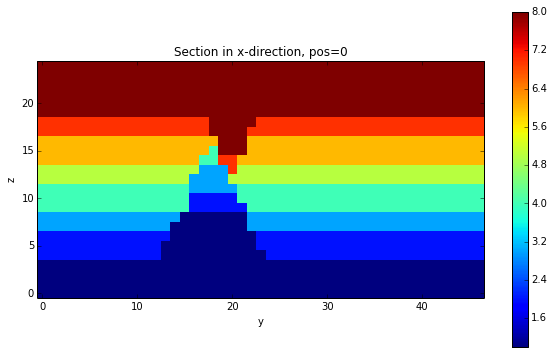
\includegraphics{1-Simulation_11_0.png}


\section{(4) Export model to VTK}
\label{notebooks/1-Simulation:export-model-to-vtk}
A simple possibility to visualise the modeled results in 3-D is to
export the model to a VTK file and then to visualise it with a VTK
viewer, for example Paraview. To export the model, simply use:

\begin{Verbatim}[commandchars=\\\{\}]
\PYG{n}{N1}\PYG{o}{.}\PYG{n}{export\PYGZus{}to\PYGZus{}vtk}\PYG{p}{(}\PYG{p}{)}
\end{Verbatim}

\begin{Verbatim}[commandchars=\\\{\}]
\PYG{k}{print}\PYG{p}{(}\PYG{l+s}{\PYGZdq{}}\PYG{l+s}{bla}\PYG{l+s}{\PYGZdq{}}\PYG{p}{)}
\end{Verbatim}

\begin{Verbatim}[commandchars=\\\{\}]
\PYG{n}{bla}
\end{Verbatim}


\chapter{Change Noddy input file and recompute model}
\label{notebooks/2-Adjust-input::doc}\label{notebooks/2-Adjust-input:change-noddy-input-file-and-recompute-model}
Visualising output of a Noddy model is nice, but not terribly helpful as
it can be done with the GUI itself. More interesting is it to change
aspects of the Noddy input (history) file with the Python module to
quickly compare the effect of changes in the geological history.

Implementing these changes in scripts is the first step to a more
extensive uncertainty analysis, as we will see in the next section.

\begin{Verbatim}[commandchars=\\\{\}]
\PYG{k+kn}{import} \PYG{n+nn}{sys}\PYG{o}{,} \PYG{n+nn}{os}
\PYG{k+kn}{import} \PYG{n+nn}{matplotlib.pyplot} \PYG{k+kn}{as} \PYG{n+nn}{plt}
\PYG{c}{\PYGZsh{} adjust some settings for matplotlib}
\PYG{k+kn}{from} \PYG{n+nn}{matplotlib} \PYG{k+kn}{import} \PYG{n}{rcParams}
\PYG{c}{\PYGZsh{} print rcParams}
\PYG{n}{rcParams}\PYG{p}{[}\PYG{l+s}{\PYGZsq{}}\PYG{l+s}{font.size}\PYG{l+s}{\PYGZsq{}}\PYG{p}{]} \PYG{o}{=} \PYG{l+m+mi}{15}
\PYG{c}{\PYGZsh{} determine path of repository to set paths corretly below}
\PYG{n}{os}\PYG{o}{.}\PYG{n}{chdir}\PYG{p}{(}\PYG{l+s}{r\PYGZsq{}}\PYG{l+s}{/Users/Florian/git/pynoddy/docs/notebooks/}\PYG{l+s}{\PYGZsq{}}\PYG{p}{)}
\PYG{n}{repo\PYGZus{}path} \PYG{o}{=} \PYG{n}{os}\PYG{o}{.}\PYG{n}{path}\PYG{o}{.}\PYG{n}{realpath}\PYG{p}{(}\PYG{l+s}{\PYGZsq{}}\PYG{l+s}{../..}\PYG{l+s}{\PYGZsq{}}\PYG{p}{)}
\PYG{k+kn}{import} \PYG{n+nn}{pynoddy}
\end{Verbatim}

First step: load the history file into a Python object:

\begin{Verbatim}[commandchars=\\\{\}]
\PYG{c}{\PYGZsh{} Change to sandbox directory to store results}
\PYG{n}{os}\PYG{o}{.}\PYG{n}{chdir}\PYG{p}{(}\PYG{n}{os}\PYG{o}{.}\PYG{n}{path}\PYG{o}{.}\PYG{n}{join}\PYG{p}{(}\PYG{n}{repo\PYGZus{}path}\PYG{p}{,} \PYG{l+s}{\PYGZsq{}}\PYG{l+s}{sandbox}\PYG{l+s}{\PYGZsq{}}\PYG{p}{)}\PYG{p}{)}

\PYG{c}{\PYGZsh{} Path to exmaple directory in this repository}
\PYG{n}{example\PYGZus{}directory} \PYG{o}{=} \PYG{n}{os}\PYG{o}{.}\PYG{n}{path}\PYG{o}{.}\PYG{n}{join}\PYG{p}{(}\PYG{n}{repo\PYGZus{}path}\PYG{p}{,}\PYG{l+s}{\PYGZsq{}}\PYG{l+s}{examples}\PYG{l+s}{\PYGZsq{}}\PYG{p}{)}
\PYG{c}{\PYGZsh{} Compute noddy model for history file}
\PYG{n}{history\PYGZus{}file} \PYG{o}{=} \PYG{l+s}{\PYGZsq{}}\PYG{l+s}{simple\PYGZus{}two\PYGZus{}faults.his}\PYG{l+s}{\PYGZsq{}}
\PYG{n}{history} \PYG{o}{=} \PYG{n}{os}\PYG{o}{.}\PYG{n}{path}\PYG{o}{.}\PYG{n}{join}\PYG{p}{(}\PYG{n}{example\PYGZus{}directory}\PYG{p}{,} \PYG{n}{history\PYGZus{}file}\PYG{p}{)}
\PYG{n}{output\PYGZus{}name} \PYG{o}{=} \PYG{l+s}{\PYGZsq{}}\PYG{l+s}{noddy\PYGZus{}out}\PYG{l+s}{\PYGZsq{}}
\PYG{n}{H1} \PYG{o}{=} \PYG{n}{pynoddy}\PYG{o}{.}\PYG{n}{NoddyHistory}\PYG{p}{(}\PYG{n}{history}\PYG{p}{)}
\end{Verbatim}


\section{(1) Get basic information on the model}
\label{notebooks/2-Adjust-input:get-basic-information-on-the-model}
The history file contains the entire information on the Noddy model.
Some information can be accessed through the NoddyHistory object (and
more will be added soon!):

\begin{Verbatim}[commandchars=\\\{\}]
\PYG{k}{pass}
\end{Verbatim}


\section{(2) Change model cube size and recompute model}
\label{notebooks/2-Adjust-input:change-model-cube-size-and-recompute-model}
The Noddy model itself is, once computed, a continuous model in 3-D
space. However, for most visualisations and further calculations (e.g.
geophysics), a discretised version is suitable. The discretisation (or
block size) can be adapted in the history file. The according pynoddy
function is change\_cube\_size.

A simple example to change the cube size and write a new history file:

\begin{Verbatim}[commandchars=\\\{\}]
\PYG{c}{\PYGZsh{} We will first recompute the model and store results in an output file for comparison}
\PYG{n+nb}{reload}\PYG{p}{(}\PYG{n}{pynoddy}\PYG{p}{)}
\PYG{n}{NH1} \PYG{o}{=} \PYG{n}{pynoddy}\PYG{o}{.}\PYG{n}{NoddyHistory}\PYG{p}{(}\PYG{n}{history}\PYG{p}{)}
\PYG{n}{pynoddy}\PYG{o}{.}\PYG{n}{compute\PYGZus{}model}\PYG{p}{(}\PYG{n}{history}\PYG{p}{,} \PYG{n}{output\PYGZus{}name}\PYG{p}{)}
\PYG{n}{NO1} \PYG{o}{=} \PYG{n}{pynoddy}\PYG{o}{.}\PYG{n}{NoddyOutput}\PYG{p}{(}\PYG{n}{output\PYGZus{}name}\PYG{p}{)}
\end{Verbatim}

\begin{Verbatim}[commandchars=\\\{\}]
\PYG{c}{\PYGZsh{} Now: change cubsize, write to new file and recompute}
\PYG{n}{NH1}\PYG{o}{.}\PYG{n}{change\PYGZus{}cube\PYGZus{}size}\PYG{p}{(}\PYG{l+m+mi}{100}\PYG{p}{)}
\PYG{c}{\PYGZsh{} Save model to a new history file and recompute (Note: may take a while to compute now)}
\PYG{n}{new\PYGZus{}history} \PYG{o}{=} \PYG{l+s}{\PYGZdq{}}\PYG{l+s}{fault\PYGZus{}model\PYGZus{}changed\PYGZus{}cubesize.his}\PYG{l+s}{\PYGZdq{}}
\PYG{n}{new\PYGZus{}output\PYGZus{}name} \PYG{o}{=} \PYG{l+s}{\PYGZdq{}}\PYG{l+s}{noddy\PYGZus{}out\PYGZus{}changed\PYGZus{}cube}\PYG{l+s}{\PYGZdq{}}
\PYG{n}{NH1}\PYG{o}{.}\PYG{n}{write\PYGZus{}history}\PYG{p}{(}\PYG{n}{new\PYGZus{}history}\PYG{p}{)}
\PYG{n}{pynoddy}\PYG{o}{.}\PYG{n}{compute\PYGZus{}model}\PYG{p}{(}\PYG{n}{new\PYGZus{}history}\PYG{p}{,} \PYG{n}{new\PYGZus{}output\PYGZus{}name}\PYG{p}{)}
\PYG{n}{NO2} \PYG{o}{=} \PYG{n}{pynoddy}\PYG{o}{.}\PYG{n}{NoddyOutput}\PYG{p}{(}\PYG{n}{new\PYGZus{}output\PYGZus{}name}\PYG{p}{)}
\end{Verbatim}

The different cell sizes are also represented in the output files:

\begin{Verbatim}[commandchars=\\\{\}]
\PYG{k}{print}\PYG{p}{(}\PYG{l+s}{\PYGZdq{}}\PYG{l+s}{Model 1 contains a total of }\PYG{l+s+si}{\PYGZpc{}7d}\PYG{l+s}{ cells with a blocksize }\PYG{l+s+si}{\PYGZpc{}.0f}\PYG{l+s}{ m}\PYG{l+s}{\PYGZdq{}} \PYG{o}{\PYGZpc{}}
      \PYG{p}{(}\PYG{n}{NO1}\PYG{o}{.}\PYG{n}{n\PYGZus{}total}\PYG{p}{,} \PYG{n}{NO1}\PYG{o}{.}\PYG{n}{delx}\PYG{p}{)}\PYG{p}{)}
\PYG{k}{print}\PYG{p}{(}\PYG{l+s}{\PYGZdq{}}\PYG{l+s}{Model 2 contains a total of }\PYG{l+s+si}{\PYGZpc{}7d}\PYG{l+s}{ cells with a blocksize }\PYG{l+s+si}{\PYGZpc{}.0f}\PYG{l+s}{ m}\PYG{l+s}{\PYGZdq{}} \PYG{o}{\PYGZpc{}}
      \PYG{p}{(}\PYG{n}{NO2}\PYG{o}{.}\PYG{n}{n\PYGZus{}total}\PYG{p}{,} \PYG{n}{NO2}\PYG{o}{.}\PYG{n}{delx}\PYG{p}{)}\PYG{p}{)}
\end{Verbatim}

\begin{Verbatim}[commandchars=\\\{\}]
Model 1 contains a total of   72850 cells with a blocksize 200 m
Model 2 contains a total of  582800 cells with a blocksize 100 m
\end{Verbatim}

We can compare the effect of the different model discretisations in
section plots, created with the plot\_section method described before.
Let's get a bit more fancy here and use the functionality to pass axes
to the plot\_section method, and to create one figure as direct
comparison:

\begin{Verbatim}[commandchars=\\\{\}]
\PYG{c}{\PYGZsh{} create basic figure layout}
\PYG{n}{fig} \PYG{o}{=} \PYG{n}{plt}\PYG{o}{.}\PYG{n}{figure}\PYG{p}{(}\PYG{n}{figsize} \PYG{o}{=} \PYG{p}{(}\PYG{l+m+mi}{15}\PYG{p}{,}\PYG{l+m+mi}{5}\PYG{p}{)}\PYG{p}{)}
\PYG{n}{ax1} \PYG{o}{=} \PYG{n}{fig}\PYG{o}{.}\PYG{n}{add\PYGZus{}subplot}\PYG{p}{(}\PYG{l+m+mi}{121}\PYG{p}{)}
\PYG{n}{ax2} \PYG{o}{=} \PYG{n}{fig}\PYG{o}{.}\PYG{n}{add\PYGZus{}subplot}\PYG{p}{(}\PYG{l+m+mi}{122}\PYG{p}{)}
\PYG{n}{NO1}\PYG{o}{.}\PYG{n}{plot\PYGZus{}section}\PYG{p}{(}\PYG{l+s}{\PYGZsq{}}\PYG{l+s}{x}\PYG{l+s}{\PYGZsq{}}\PYG{p}{,} \PYG{n}{ax} \PYG{o}{=} \PYG{n}{ax1}\PYG{p}{,} \PYG{n}{colorbar}\PYG{o}{=}\PYG{n+nb+bp}{False}\PYG{p}{,} \PYG{n}{title}\PYG{o}{=}\PYG{l+s}{\PYGZdq{}}\PYG{l+s}{Model 1}\PYG{l+s}{\PYGZdq{}}\PYG{p}{)}
\PYG{n}{NO2}\PYG{o}{.}\PYG{n}{plot\PYGZus{}section}\PYG{p}{(}\PYG{l+s}{\PYGZsq{}}\PYG{l+s}{x}\PYG{l+s}{\PYGZsq{}}\PYG{p}{,} \PYG{n}{ax} \PYG{o}{=} \PYG{n}{ax2}\PYG{p}{,} \PYG{n}{colorbar}\PYG{o}{=}\PYG{n+nb+bp}{False}\PYG{p}{,} \PYG{n}{title}\PYG{o}{=}\PYG{l+s}{\PYGZdq{}}\PYG{l+s}{Model 2}\PYG{l+s}{\PYGZdq{}}\PYG{p}{)}

\PYG{n}{plt}\PYG{o}{.}\PYG{n}{show}\PYG{p}{(}\PYG{p}{)}
\end{Verbatim}

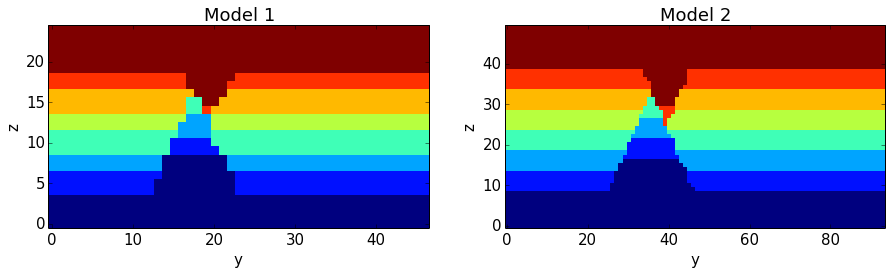
\includegraphics{2-Adjust-input_12_0.png}


\section{(3) Change aspects of geological events}
\label{notebooks/2-Adjust-input:change-aspects-of-geological-events}
Ok, now from some basic settings to the things that we actually want to
change: aspects of the geological history defined in Noddy. This can
happen on two hierarchical levels: on the level of each single event
(i.e. changing parameters relating to one event) and on the level of the
events themselves (i.e. the order of the events).

We will here have a look at the paramteres of the single events:


\chapter{Indices and tables}
\label{index:indices-and-tables}\begin{itemize}
\item {} 
\emph{genindex}

\item {} 
\emph{modindex}

\item {} 
\emph{search}

\end{itemize}


\renewcommand{\indexname}{Python Module Index}
\begin{theindex}
\def\bigletter#1{{\Large\sffamily#1}\nopagebreak\vspace{1mm}}
\bigletter{p}
\item {\texttt{pynoddy}}, \pageref{pynoddy:module-pynoddy}
\item {\texttt{pynoddy.history}}, \pageref{pynoddy:module-pynoddy.history}
\item {\texttt{pynoddy.output}}, \pageref{pynoddy:module-pynoddy.output}
\end{theindex}

\renewcommand{\indexname}{Index}
\printindex
\end{document}
